\documentclass[12pt,a4paper,openany,oneside]{report}
\usepackage[utf8]{vietnam}
\usepackage{amsmath, amsthm, amssymb,amsxtra,latexsym,amscd,graphpap,makeidx}
\usepackage{pgf,tikz}
\usepackage{mathrsfs}
\usetikzlibrary{arrows}
\usepackage{float}
\usepackage{algorithm}
\usepackage{algpseudocode}
\usepackage{graphicx}
\usepackage{array,tabularx,longtable,multicol,indentfirst,fancyhdr}%
\usepackage[mathscr]{eucal}
\usepackage[top=3.5cm, bottom=3.0cm, left=3.5cm, right=2cm] {geometry}
\usepackage{fancybox}
\usepackage{listings}
\usepackage{xcolor}
\usepackage[utf8]{inputenc}

% Định dạng code Python
\definecolor{codegreen}{rgb}{0,0.6,0}
\definecolor{codegray}{rgb}{0.5,0.5,0.5}
\definecolor{codepurple}{rgb}{0.58,0,0.82}
\definecolor{backcolour}{rgb}{0.95,0.95,0.92}

\lstdefinestyle{mystyle}{
    backgroundcolor=\color{backcolour},   
    commentstyle=\color{codegreen},
    keywordstyle=\color{magenta},
    numberstyle=\tiny\color{codegray},
    stringstyle=\color{codepurple},
    basicstyle=\ttfamily\footnotesize,
    breakatwhitespace=false,         
    breaklines=true,                 
    captionpos=b,                    
    keepspaces=true,                 
    numbers=left,                    
    numbersep=5pt,                  
    showspaces=false,                
    showstringspaces=false,
    showtabs=false,                  
    tabsize=2,
    inputencoding=utf8,
    extendedchars=true,
    literate={á}{{\'a}}1 {é}{{\'e}}1 {í}{{\'i}}1 {ó}{{\'o}}1 {ú}{{\'u}}1
      {Á}{{\'A}}1 {É}{{\'E}}1 {Í}{{\'I}}1 {Ó}{{\'O}}1 {Ú}{{\'U}}1
      {à}{{\`a}}1 {è}{{\`e}}1 {ì}{{\`i}}1 {ò}{{\`o}}1 {ù}{{\`u}}1
      {À}{{\`A}}1 {È}{{\'E}}1 {Ì}{{\`I}}1 {Ò}{{\`O}}1 {Ù}{{\`U}}1
      {ä}{{\"a}}1 {ë}{{\"e}}1 {ï}{{\"i}}1 {ö}{{\"o}}1 {ü}{{\"u}}1
      {Ä}{{\"A}}1 {Ë}{{\"E}}1 {Ï}{{\"I}}1 {Ö}{{\"O}}1 {Ü}{{\"U}}1
      {â}{{\^a}}1 {ê}{{\^e}}1 {î}{{\^i}}1 {ô}{{\^o}}1 {û}{{\^u}}1
      {Â}{{\^A}}1 {Ê}{{\^E}}1 {Î}{{\^I}}1 {Ô}{{\^O}}1 {Û}{{\^U}}1
      {œ}{{\oe}}1 {Œ}{{\OE}}1 {æ}{{\ae}}1 {Æ}{{\AE}}1 {ß}{{\ss}}1
      {ç}{{\c c}}1 {Ç}{{\c C}}1 {ø}{{\o}}1 {å}{{\r a}}1 {Å}{{\r A}}1
      {ã}{{\~a}}1 {õ}{{\~o}}1 {Ã}{{\~A}}1 {Õ}{{\~O}}1
      {ñ}{{\~n}}1 {Ñ}{{\~N}}1 {¿}{{?`}}1 {¡}{{!`}}1
      {°}{{\textdegree}}1 {ð}{{\dh}}1 {Ð}{{\DH}}1 {þ}{{\th}}1 {Þ}{{\TH}}1
}

\lstset{style=mystyle}

%==================================  
\newtheorem{dl}{Định lý}[section]
\newtheorem{dn}[dl]{Định nghĩa} 
\newtheorem{bt}[dl]{Bài toán} 
\newtheorem{btp}[dl]{Bài tập} 
\newtheorem{bta}[dl]{Bài} 
\newtheorem{bai}[dl]{Bài}
\newtheorem{tc}[dl]{Tính chất} 
\newtheorem{md}[dl]{Mệnh đề} 
\newtheorem{bd}[dl]{Bổ đề} 
\newtheorem{hq}[dl]{Hệ quả} 
\newtheorem{nx}[dl]{Nhận xét} 
\newtheorem{cy}[dl]{Chú ý} 
\newtheorem{vd}[dl]{Ví dụ} 
\usepackage{hyperref}
\renewcommand{\chaptername}{Chương \chaptername}
\renewcommand\bibname{Tài liệu tham khảo}
%.....................................

\newcommand{\bpr}{\begin{proof}}
\newcommand{\epr}{\end{proof}}

 % package content table

%-----------------------------------------------
\def\en{\enskip}
\def\n{\noindent}
\def\m{\medskip}
\def\en{\enskip}
\def\m{\medskip}
\def\n{\noindent}
\def\Re{\mbox{Re }}
\def\Im{\mbox{Im }}
\def\hcm{\hfill $\square$\\}
\def\imotn{i = 1, 2, \ldots, n}
\def\ii{\item}


\def\N{\mathbb{N}}
\def\Z{\mathbb{Z}}
\def\R{\mathbb{R}}
\def\Q{\mathbb{Q}}
\def\C{\mathscr{C}}  
\def\K{\mathbb{K}}  
\def\F{\mathbb{F}}  
\def\L{\mathbb{L}} 
\DeclareMathOperator{\ord}{ord}

\allowdisplaybreaks
\newenvironment{giai}{\noindent{\em \textit{Giải}. }}{\hfill $\square$}

%%%%%%%%%%%%%%%%%%%%%%%%%%%% 
 
\makeatletter 
\renewcommand{\ps@plain}{
    \renewcommand{\@oddhead}{\hfil{\thepage}\hfil}
    \renewcommand{\@evenhead}{\@oddhead}
    \renewcommand{\@oddfoot}{\empty}
    \renewcommand{\@evenfoot}{\@oddfoot}   }
\makeatother
\pagestyle{fancy}
\fancyhf{}
\rhead{}
\chead{\normalsize  \thepage}
\lhead{\itshape {\nouppercase{}}}
\renewcommand{\headrulewidth}{0pt}

\begin{document}
	
	%Cô mới thêm vào đoạn này
	%========================================
	\pagestyle{fancy}
	\fancyhf{}
	\fancyhead[L]{BÁO CÁO BÀI TẬP LỚN} % Di chuyển header về bên trái
	\renewcommand{\headrulewidth}{0.4pt} % Gạch dưới header
	\fancyfoot[L]{Nguyễn Trường Thái - DXHTTTY }
	\fancyfoot[R]{\roman{page}} % Số trang theo chữ số La mã ở bên phải của footer
	\renewcommand{\footrulewidth}{0.4pt} % Dòng kẻ trên footer
	
	\pagenumbering{gobble}
	
	%==============================================
%\pagenumbering{roman}

\newgeometry{top=2.0cm,bottom=3.0cm,left=3.0cm,right=2.8cm}
\setlength{\fboxrule}{1.5pt}
\thisfancypage{\setlength{\fboxsep}{10pt}\setlength{\shadowsize}{0pt}\doublebox}{}

\begin{titlepage}
\fontsize{14pt}{14pt}\selectfont \baselineskip 0.65cm
\thispagestyle{empty}
\begin{center}
{HỌC VIỆN CÔNG NGHỆ BƯU CHÍNH VIỄN THÔNG}\\
\textbf{\MakeUppercase{KHOA CÔNG NGHỆ THÔNG TIN I}}\\
\centerline{--------------------o0o--------------------}  
\end{center}
 

\begin{figure}[H]
	\begin{center}
		
\includegraphics[width=6cm]{./logo}
	\end{center}
\end{figure} 
 
 
\vspace{0.5cm}
\begin{center}
\textbf{\MakeUppercase{\LARGE \bf BÁO CÁO BÀI TẬP LỚN}}\\ 
\end{center} 

\vspace{1cm}
\begin{center}
	Đề tài: 
	\textbf{\MakeUppercase{ \bf ``THUẬT TOÁN PRM (PROBABILISTIC ROADMAP) VÀ ỨNG DỤNG TRONG LẬP TRÌNH DI CHUYỂN ROBOT''}}\\ 
\end{center} 
\vspace{2cm}


\begin{tabular}{ll}
	{\textbf{\large{Giảng Viên Hướng Dẫn: }}} & {\textbf{\large{TS. Nguyễn Kiều Linh}}} \\
	{\textbf{\large{Sinh viên thực hiện:}}}  & {\textbf{\large{Nguyễn Trường Thái}}} \\
	{\textbf{\large{Mã sinh viên: }}}  & {\textbf{\large{BXXDCCNYYY}}} \\
	{\textbf{\large{Lớp:}}}   & {\textbf{\large{DXHTTTY}}}\\
	{\textbf{\large{Niên khóa:}}}   & {\textbf{\large{20xx-20xx}}}\\
	{\textbf{\large{Hệ đào tạo:}}}   & {\textbf{\large{Đại học chính quy}}}
\end{tabular}

\vfill
\begin{center}
{{\bf Hà Nội, 4/2025}}
\end{center}
\end{titlepage}

\newgeometry{top=2.0cm,bottom=3.0cm,left=3.0cm,right=2.8cm}
\setlength{\fboxrule}{1.5pt}
\thisfancypage{\setlength{\fboxsep}{10pt}\setlength{\shadowsize}{0pt}\doublebox}{}

\fontsize{14pt}{14pt}\selectfont \baselineskip 0.65cm
\thispagestyle{empty}
\begin{center}
	{HỌC VIỆN CÔNG NGHỆ BƯU CHÍNH VIỄN THÔNG}\\
	\textbf{\MakeUppercase{KHOA CÔNG NGHỆ THÔNG TIN I}}\\
	\centerline{--------------------o0o--------------------}  
\end{center}


\begin{figure}[H]
	\begin{center}
		
\includegraphics[width=6cm]{./logo}
	\end{center}
\end{figure} 

\vspace{0.5cm}
\begin{center}
	\textbf{\MakeUppercase{\LARGE \bf BÁO CÁO BÀI TẬP LỚN}}\\ 
\end{center} 

\vspace{1cm}
\begin{center}
\textbf{Đề tài:}
	\textbf{\MakeUppercase{ \bf ``THUẬT TOÁN PRM (PROBABILISTIC ROADMAP) VÀ ỨNG DỤNG TRONG LẬP TRÌNH DI CHUYỂN ROBOT''}}\\ 
\end{center} 
\vspace{2cm}


\begin{tabular}{ll}
	{\textbf{\large{Giảng Viên Hướng Dẫn: }}} & {\large TS. Nguyễn Kiều Linh}\\
	{\textbf{\large{Sinh viên thực hiện:}}}  & {\large Nguyễn Trường Thái} \\
	{\textbf{\large{Mã sinh viên: }}}  & {\large BXXDCCNYYY} \\
	{\textbf{\large{Lớp:}}}   & {\large DXHTTTY}\\
	{\textbf{\large{Niên khóa:}}}   & {\large 20xx-20xx}\\
	{\textbf{\large{Hệ đào tạo:}}}   & {\large Đại học chính quy}
\end{tabular}


\vfill
\begin{center}
	{{\bf Hà Nội, 4/2025}}
\end{center}

%Cô mới thêm vào đoạn này
%========================================

%%%%%%%%%%%%%%%
\newgeometry{top=2.5cm,bottom=2cm,left=3cm,right=2cm} 
\thispagestyle{empty}
\begin{center}
	{\textbf{\Large{NHẬN XÉT CỦA GIẢNG VIÊN HƯỚNG DẪN}}}
\end{center}

\dotfill \vspace{0.25cm} \par
\dotfill \vspace{0.25cm} \par
\dotfill \vspace{0.25cm} \par
\dotfill \vspace{0.25cm} \par
\dotfill \vspace{0.25cm} \par
\dotfill \vspace{0.25cm} \par
\dotfill \vspace{0.25cm} \par
\dotfill \vspace{0.25cm} \par
\dotfill \vspace{0.25cm} \par
\dotfill \vspace{0.25cm} \par
\dotfill \vspace{0.25cm} \par
\dotfill \vspace{0.25cm} \par
\dotfill \vspace{0.25cm} \par
\dotfill \vspace{0.25cm} \par
\dotfill \vspace{0.25cm} \par
\dotfill \vspace{0.25cm} \par
\dotfill \vspace{0.25cm} \par
\dotfill \vspace{0.25cm} \par
\dotfill

\vspace{1cm}

{\textbf{\large{Điểm: }}} \hspace{1.0cm}\textbf{( Bằng chữ:}  \hspace{2.5cm}\textbf{)}  

\begin{flushright}
	Hà Nội, ngày \hspace{0.75cm} tháng \hspace{0.75cm} năm 20...\hspace{0.75cm}
	
	{\textbf{\large{Giảng viên hướng dẫn }}} \hspace{1cm} \textcolor{white}{.}
\end{flushright}

\newgeometry{top=2.5cm,bottom=2cm,left=3cm,right=2cm} 
\thispagestyle{empty}
\begin{center}
	{\textbf{\Large{NHẬN XÉT CỦA GIẢNG VIÊN PHẢN BIỆN}}}
\end{center}

\dotfill \vspace{0.25cm} \par
\dotfill \vspace{0.25cm} \par
\dotfill \vspace{0.25cm} \par
\dotfill \vspace{0.25cm} \par
\dotfill \vspace{0.25cm} \par
\dotfill \vspace{0.25cm} \par
\dotfill \vspace{0.25cm} \par
\dotfill \vspace{0.25cm} \par
\dotfill \vspace{0.25cm} \par
\dotfill \vspace{0.25cm} \par
\dotfill \vspace{0.25cm} \par
\dotfill \vspace{0.25cm} \par
\dotfill \vspace{0.25cm} \par
\dotfill \vspace{0.25cm} \par
\dotfill \vspace{0.25cm} \par
\dotfill \vspace{0.25cm} \par
\dotfill \vspace{0.25cm} \par
\dotfill \vspace{0.25cm} \par
\dotfill

\vspace{1cm}

{\textbf{\large{Điểm: }}} \hspace{1.0cm}\textbf{( Bằng chữ:}  \hspace{2.5cm}\textbf{)}  

\begin{flushright}
	Hà Nội, ngày \hspace{0.75cm} tháng \hspace{0.75cm} năm 20...\hspace{0.75cm}
	
	{\textbf{\large{Giảng viên phản biện }}} \hspace{1cm} \textcolor{white}{.}
\end{flushright}

%==============================================

\restoregeometry
\pagestyle{fancy}
\pagenumbering{roman}
\fontsize{13pt}{13pt}\selectfont \baselineskip 0.75cm 

\newpage
\thispagestyle{empty}
%\thispagestyle{fancy}
%\pagenumbering{roman}
%\vspace*{-2.5cm} % Thay đổi giá trị để điều chỉnh khoảng cách
% Tạo mục lục tự động
%\addcontentsline{toc}{chapter}{Mục lục}
\tableofcontents

%%%%%%%%%%%%%%%%%%%
\newpage
\begin{center}
	\Large{\textbf{LỜI CẢM ƠN}}\\
\end{center}
\vspace{1cm}

Trước hết, tôi xin gửi lời cảm ơn chân thành và sâu sắc đến TS. Nguyễn Kiều Linh, người đã tận tình hướng dẫn, chỉ bảo và hỗ trợ tôi trong suốt quá trình thực hiện đồ án này. Những kiến thức, kinh nghiệm và sự nhiệt tình của cô đã giúp tôi hoàn thành đồ án một cách tốt nhất.

Tôi cũng xin gửi lời cảm ơn đến các thầy cô giáo trong Khoa Công nghệ Thông tin I, Học viện Công nghệ Bưu chính Viễn thông, những người đã truyền đạt kiến thức, kỹ năng và tạo điều kiện thuận lợi cho tôi trong suốt quá trình học tập và nghiên cứu.

Cuối cùng, tôi xin cảm ơn gia đình, bạn bè đã luôn bên cạnh, động viên và hỗ trợ tôi trong suốt thời gian qua.

\phantom{nnnnnnnnnnnnnnnnnnnnnnnnnnnnnnn}\  {\textit{Hà Nội, tháng 4 năm 2025}} \\
\phantom{nnnnnnnnnnnnnnnnnnnnnnnnnnnnnnnnnnnnnnnnn} {Sinh viên}\\
\phantom{nnnnnnnnnnnnnnnnnnnnnnnnnnnnnnnnnn} \\
\phantom{nnnnnnnnnnnnnnnnnnnnnnnnnnnnnnnnnn} \\ 
\phantom{nnnnnnnnnnnnnnnnnnnnnnnnnnnnnnnnnn} \\ 
\phantom{nnnnnnnnnnnnnnnnnnnnnnnnnnnnnnnnnnnnnnn}   {Nguyễn Trường Thái}

%%%%%%%%%%%%%%%%%%%%%%%%%%%%

\newpage 
\addcontentsline{toc}{chapter}{\bf  Danh sách hình vẽ} 

\listoffigures

%%%%%%%%%%%%%%%%%%%%%%%%%%%%

\newpage 
\addcontentsline{toc}{chapter}{\bf  Danh sách bảng} 
\listoftables

%%%%%%%%%%%%%%%%%%%%%%%%%%%%
	\newpage
{\addcontentsline{toc}{chapter}{Danh sách các ký hiệu và chữ viết tắt}}

\begin{center}
	{\LARGE
		{\bf Danh sách các ký hiệu và chữ viết tắt}}
\end{center}
\vspace{1.25cm}
{\fontsize{13}{13}\selectfont
	\begin{tabular}{ll}
		PRM & Probabilistic Roadmap (Bản đồ xác suất)\\
		RRT & Rapidly-exploring Random Tree (Cây ngẫu nhiên khám phá nhanh)\\
		KNN & K-Nearest Neighbors (K láng giềng gần nhất)\\
		UAV & Unmanned Aerial Vehicle (Phương tiện bay không người lái)\\
		KDTree & K-Dimensional Tree (Cấu trúc dữ liệu cây K chiều)\\
	\end{tabular}
}

\newpage
\pagenumbering{arabic} 
\pagestyle{fancy} 

\chapter*{Mở đầu}
\addcontentsline{toc}{chapter}{Mở đầu} 

Trong lĩnh vực robotics, một trong những thách thức cơ bản là làm thế nào để robot có thể di chuyển an toàn và hiệu quả trong môi trường có chướng ngại vật. Bài toán này, được gọi là bài toán lập kế hoạch đường đi (path planning), đóng vai trò quan trọng trong nhiều ứng dụng thực tế như robot công nghiệp, xe tự hành, thiết bị bay không người lái (UAV), và robot phẫu thuật.

Trong số nhiều phương pháp giải quyết bài toán lập kế hoạch đường đi, thuật toán PRM (Probabilistic Roadmap) nổi bật như một giải pháp hiệu quả, đặc biệt trong môi trường phức tạp với nhiều chướng ngại vật. Thuật toán này dựa trên nguyên lý xác suất, tạo ra một "bản đồ đường đi" bằng cách sinh ngẫu nhiên các điểm trong không gian tự do và kết nối chúng lại với nhau, sau đó sử dụng các thuật toán tìm đường như Dijkstra hoặc A* để tìm đường đi tối ưu từ điểm xuất phát đến điểm đích.

Đồ án này tập trung nghiên cứu về thuật toán PRM, từ cơ sở lý thuyết đến triển khai thực tế trong lập trình di chuyển robot. Chúng tôi sẽ phân tích chi tiết các giai đoạn của thuật toán, cài đặt thuật toán bằng ngôn ngữ Python, và minh họa kết quả thông qua các hình ảnh trực quan. Ngoài ra, đồ án cũng so sánh PRM với các thuật toán lập kế hoạch đường đi khác như RRT (Rapidly-exploring Random Tree) và RRT*, đồng thời thảo luận về các ứng dụng thực tế của PRM trong nhiều lĩnh vực.

Mục tiêu của đồ án là cung cấp một cái nhìn toàn diện về thuật toán PRM, giúp người đọc hiểu rõ cách thức hoạt động, ưu nhược điểm, và tiềm năng ứng dụng của thuật toán này trong việc giải quyết bài toán lập kế hoạch đường đi cho robot.

\chapter{Tổng quan về thuật toán PRM}

\section{Giới thiệu về bài toán lập kế hoạch đường đi}

Lập kế hoạch đường đi (path planning) là một trong những bài toán cơ bản và quan trọng trong lĩnh vực robotics. Bài toán này đặt ra yêu cầu tìm một đường đi từ điểm xuất phát đến điểm đích, tránh các chướng ngại vật trong môi trường, và tối ưu hóa theo một số tiêu chí như khoảng cách, thời gian, hoặc năng lượng tiêu thụ.

Bài toán lập kế hoạch đường đi có nhiều ứng dụng thực tế trong các lĩnh vực như:
\begin{itemize}
    \item Robot công nghiệp trong nhà máy
    \item Xe tự hành trên đường phố
    \item Thiết bị bay không người lái (UAV)
    \item Robot phẫu thuật trong y tế
    \item Robot dịch vụ trong khách sạn, nhà hàng
\end{itemize}

Có nhiều phương pháp để giải quyết bài toán lập kế hoạch đường đi, từ các phương pháp cổ điển như thuật toán A*, Dijkstra đến các phương pháp hiện đại dựa trên xác suất như PRM, RRT. Mỗi phương pháp đều có những ưu điểm và hạn chế riêng, phù hợp với các tình huống và yêu cầu khác nhau.

\section{Khái niệm và nguyên lý của thuật toán PRM}

Thuật toán PRM (Probabilistic Roadmap) là một phương pháp lập kế hoạch đường đi dựa trên xác suất, được giới thiệu lần đầu bởi Kavraki và cộng sự vào năm 1996. Thuật toán này hoạt động dựa trên nguyên lý tạo ra một "bản đồ đường đi" (roadmap) bằng cách sinh ngẫu nhiên các điểm trong không gian tự do và kết nối chúng lại với nhau.

Nguyên lý cơ bản của thuật toán PRM bao gồm hai giai đoạn chính:

\begin{enumerate}
    \item \textbf{Giai đoạn xây dựng bản đồ (Learning Phase):} Trong giai đoạn này, thuật toán sinh ngẫu nhiên các điểm trong không gian tự do (không có chướng ngại vật), sau đó kết nối các điểm gần nhau bằng các cạnh nếu đường nối giữa chúng không đi qua chướng ngại vật. Kết quả là một đồ thị với các đỉnh là các điểm mẫu và các cạnh là các đường nối khả thi.
    
    \item \textbf{Giai đoạn truy vấn (Query Phase):} Khi có yêu cầu tìm đường từ điểm xuất phát đến điểm đích, thuật toán sẽ kết nối hai điểm này vào bản đồ đã xây dựng, sau đó sử dụng các thuật toán tìm đường trên đồ thị như Dijkstra hoặc A* để tìm đường đi tối ưu.
\end{enumerate}

Thuật toán PRM có một số ưu điểm nổi bật:
\begin{itemize}
    \item Hiệu quả trong không gian có nhiều chiều
    \item Khả năng xử lý môi trường phức tạp với nhiều chướng ngại vật
    \item Giai đoạn xây dựng bản đồ chỉ cần thực hiện một lần, sau đó có thể sử dụng lại cho nhiều truy vấn khác nhau
    \item Dễ dàng mở rộng và tùy chỉnh cho các ứng dụng cụ thể
\end{itemize}

\section{So sánh PRM với các thuật toán lập kế hoạch đường đi khác}

Để hiểu rõ hơn về vị trí và vai trò của thuật toán PRM trong lĩnh vực lập kế hoạch đường đi, chúng ta cần so sánh nó với các thuật toán khác, đặc biệt là RRT (Rapidly-exploring Random Tree) và RRT*.

\begin{table}[h]
\centering
\begin{tabular}{|p{2cm}|p{4cm}|p{4cm}|p{4cm}|}
\hline
\textbf{Thuật toán} & \textbf{Cách hoạt động} & \textbf{Ưu điểm} & \textbf{Nhược điểm} \\
\hline
PRM & Tạo đồ thị toàn cục trước rồi tìm đường & Nhanh với không gian tĩnh, nhiều lần dùng & Không hợp với robot động học phức tạp \\
\hline
RRT & Tạo cây từ start, mở rộng dần & Dễ dùng với không gian động, đơn giản & Đường đi xấu, không tối ưu \\
\hline
RRT* & Giống RRT, nhưng tối ưu hóa cây & Đường đi tốt hơn, gần tối ưu & Chậm hơn, phức tạp hơn \\
\hline
\end{tabular}
\caption{So sánh các thuật toán lập kế hoạch đường đi}
\label{tab:comparison}
\end{table}

\textbf{PRM vs RRT:}
\begin{itemize}
    \item PRM xây dựng một đồ thị toàn cục, trong khi RRT xây dựng một cây từ điểm xuất phát.
    \item PRM phù hợp với môi trường tĩnh và nhiều truy vấn, trong khi RRT phù hợp với môi trường động và truy vấn đơn.
    \item PRM yêu cầu nhiều tính toán trong giai đoạn xây dựng bản đồ, nhưng nhanh trong giai đoạn truy vấn, trong khi RRT phân bố tính toán đều hơn.
\end{itemize}

\textbf{PRM vs RRT*:}
\begin{itemize}
    \item RRT* là phiên bản cải tiến của RRT, tập trung vào việc tối ưu hóa đường đi.
    \item PRM thường cho kết quả tối ưu hơn RRT, nhưng có thể không tối ưu bằng RRT* khi số lượng điểm mẫu tương đương.
    \item RRT* có khả năng hội tụ đến đường đi tối ưu khi số lượng điểm mẫu tăng lên, trong khi PRM không đảm bảo điều này.
\end{itemize}

\textbf{Yêu cầu và hạn chế của PRM:}
\begin{itemize}
    \item PRM đòi hỏi map tĩnh do các nguyên nhân sau:
    \begin{itemize}
        \item Đồ thị được xây dựng trước (offline) dựa trên vị trí chướng ngại vật cố định
        \item Mọi thay đổi về vị trí vật cản đòi hỏi xây dựng lại toàn bộ roadmap
        \item Thuật toán không có cơ chế cập nhật động các kết nối đã tồn tại
    \end{itemize}
    
    \item Hạn chế chính:
    \begin{itemize}
        \item Hiệu suất giảm mạnh trong không gian nhiều chiều
        \item Khó xử lý các chướng ngại vật di động hoặc thay đổi hình dạng
        \item Phụ thuộc nhiều vào chất lượng phân bố điểm mẫu ban đầu
    \end{itemize}
\end{itemize}

\chapter{Triển khai thuật toán PRM}

\section{Các giai đoạn của thuật toán PRM}

Thuật toán PRM được triển khai qua bốn giai đoạn chính, mỗi giai đoạn đóng vai trò quan trọng trong việc xây dựng bản đồ đường đi và tìm đường đi tối ưu.

\subsection{Giai đoạn 1: Ghi nhớ bản đồ (vật cản)}

Giai đoạn đầu tiên của thuật toán PRM là ghi nhớ bản đồ môi trường, bao gồm vị trí của các chướng ngại vật, điểm xuất phát và điểm đích. Đây là bước quan trọng để xác định không gian tự do mà robot có thể di chuyển.

\begin{figure}[H]
    \centering
    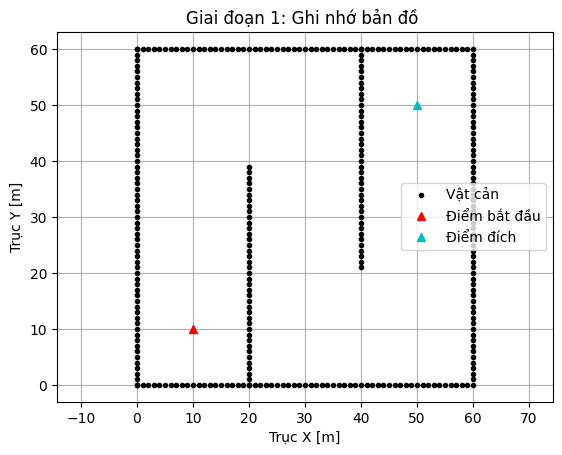
\includegraphics[width=0.8\textwidth]{giai_doan_1}
    \caption{Giai đoạn 1: Ghi nhớ bản đồ với vật cản, điểm bắt đầu và điểm đích}
    \label{fig:stage1}
\end{figure}

Trong hình \ref{fig:stage1}, chúng ta có thể thấy:
\begin{itemize}
    \item Các chấm đen biểu thị vị trí của các chướng ngại vật
    \item Tam giác đỏ biểu thị điểm xuất phát
    \item Tam giác xanh biểu thị điểm đích
\end{itemize}

Môi trường trong ví dụ này là một không gian 2D với các chướng ngại vật được bố trí theo hình dạng của một mê cung đơn giản. Robot cần tìm đường đi từ điểm xuất phát ở góc dưới bên trái đến điểm đích ở phía trên bên phải.

\subsection{Giai đoạn 2: Tạo điểm mẫu}

Sau khi đã ghi nhớ bản đồ môi trường, thuật toán PRM tiến hành sinh ngẫu nhiên các điểm mẫu trong không gian tự do. Các điểm này sẽ trở thành các đỉnh của đồ thị bản đồ đường đi.

\begin{figure}[H]
    \centering
    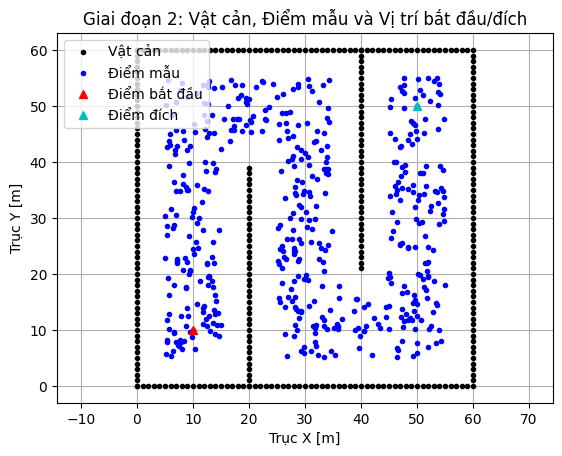
\includegraphics[width=0.8\textwidth]{giai_doan_2}
    \caption{Giai đoạn 2: Tạo điểm mẫu trong không gian tự do}
    \label{fig:stage2}
\end{figure}

Trong hình \ref{fig:stage2}, chúng ta có thể thấy:
\begin{itemize}
    \item Các chấm xanh biểu thị các điểm mẫu được sinh ngẫu nhiên trong không gian tự do
    \item Các điểm mẫu được phân bố đều trong toàn bộ không gian tự do, bao gồm cả các khu vực hẹp và rộng
\end{itemize}

Quá trình sinh điểm mẫu tuân theo một số nguyên tắc:
\begin{itemize}
    \item Các điểm mẫu phải nằm trong không gian tự do, tức là không nằm trong hoặc quá gần các chướng ngại vật
    \item Số lượng điểm mẫu phải đủ lớn để đảm bảo khả năng tìm được đường đi, nhưng không quá lớn để tránh tốn kém về mặt tính toán
    \item Phân bố của các điểm mẫu nên đều trong không gian tự do để đảm bảo khả năng tìm được đường đi tối ưu
\end{itemize}

\subsection{Giai đoạn 3: Duyệt nút và đánh dấu}

Sau khi đã sinh các điểm mẫu, thuật toán PRM tiến hành kết nối các điểm này để tạo thành một đồ thị. Mỗi điểm sẽ được kết nối với một số điểm gần nhất nếu đường nối giữa chúng không đi qua chướng ngại vật.

\begin{figure}[H]
    \centering
    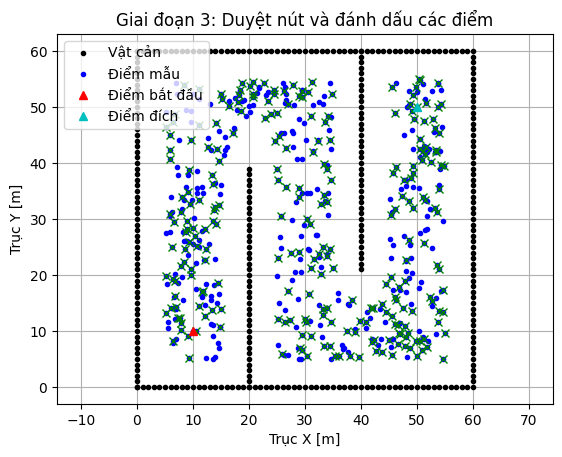
\includegraphics[width=0.8\textwidth]{giai_doan_3}
    \caption{Giai đoạn 3: Duyệt nút và đánh dấu các kết nối}
    \label{fig:stage3}
\end{figure}

Trong hình \ref{fig:stage3}, chúng ta có thể thấy:
\begin{itemize}
    \item Các chấm xanh vẫn biểu thị các điểm mẫu
    \item Các dấu "x" xanh lá biểu thị các kết nối giữa các điểm mẫu
\end{itemize}

Quá trình kết nối các điểm mẫu tuân theo một số nguyên tắc:
\begin{itemize}
    \item Mỗi điểm sẽ được kết nối với K điểm gần nhất (K-Nearest Neighbors)
    \item Một kết nối chỉ được tạo ra nếu đường thẳng nối hai điểm không đi qua chướng ngại vật
    \item Độ dài của một kết nối không vượt quá một ngưỡng cho trước để tránh tạo ra các kết nối quá dài và không thực tế
\end{itemize}

\subsection{Giai đoạn 4: Kết quả đường đi tối ưu}

Giai đoạn cuối cùng của thuật toán PRM là tìm đường đi tối ưu từ điểm xuất phát đến điểm đích trên đồ thị đã xây dựng. Thuật toán sử dụng Dijkstra hoặc A* để tìm đường đi ngắn nhất.

\begin{figure}[H]
    \centering
    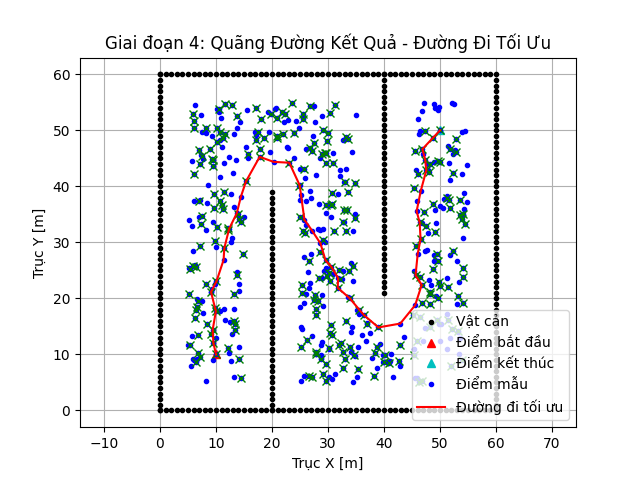
\includegraphics[width=0.8\textwidth]{giai_doan_4}
    \caption{Giai đoạn 4: Kết quả đường đi tối ưu}
    \label{fig:stage4}
\end{figure}

Trong hình \ref{fig:stage4}, chúng ta có thể thấy:
\begin{itemize}
    \item Đường màu đỏ biểu thị đường đi tối ưu từ điểm xuất phát đến điểm đích
    \item Đường đi này đi qua các điểm mẫu và tránh các chướng ngại vật
\end{itemize}

Đường đi tối ưu được tìm thấy bằng cách:
\begin{itemize}
    \item Kết nối điểm xuất phát và điểm đích vào đồ thị bản đồ đường đi
    \item Sử dụng thuật toán Dijkstra để tìm đường đi ngắn nhất từ điểm xuất phát đến điểm đích
    \item Làm mịn đường đi nếu cần thiết để tạo ra một đường đi trơn tru và tự nhiên hơn
\end{itemize}

\section{Cài đặt thuật toán PRM bằng Python}

Dưới đây là cài đặt chi tiết của thuật toán PRM bằng ngôn ngữ Python, sử dụng các thư viện NumPy, Matplotlib và SciPy.

\begin{lstlisting}[language=Python, caption=Cài đặt thuật toán PRM bằng Python]
import math
import numpy as np
import matplotlib.pyplot as plt
from scipy.spatial import KDTree

# Cau hinh co ban
N_SAMPLE = 500  # So diem lay mau
N_KNN = 10      # So hang xom gan nhat de ket noi
MAX_EDGE_LEN = 30.0  # Do dai cung toi da

show_animation = True  # Hien thi hoat hinh

# Lop Nut luu thong tin diem
class Node:
    def __init__(self, x, y, cost, parent_index):
        self.x = x  # Toa do x
        self.y = y  # Toa do y
        self.cost = cost  # Chi phi den diem nay
        self.parent_index = parent_index  # Chi so diem cha

    def __str__(self):
        return str(self.x) + "," + str(self.y) + "," + str(self.cost) + "," + str(self.parent_index)

# Ham chinh lap ke hoach duong di PRM
def prm_planning(start_x, start_y, goal_x, goal_y,
                 obstacle_x_list, obstacle_y_list, robot_radius):
    
    obstacle_kd_tree = KDTree(np.vstack((obstacle_x_list, obstacle_y_list)).T)  # Tao KDTree cho vat can

    sample_x, sample_y = sample_points(
        start_x, start_y, goal_x, goal_y,
        robot_radius,
        obstacle_x_list, obstacle_y_list,
        obstacle_kd_tree
    )  # Lay mau diem

    if show_animation:
        plt.plot(sample_x, sample_y, ".b")  # Ve diem lay mau

    road_map = generate_road_map(sample_x, sample_y, robot_radius, obstacle_kd_tree)  # Tao ban do duong di

    rx, ry = dijkstra_planning(start_x, start_y, goal_x, goal_y, road_map, sample_x, sample_y)  # Tim duong di ngan nhat

    return rx, ry

# Lay mau diem trong khong gian
def sample_points(sx, sy, gx, gy, rr, ox, oy, obstacle_kd_tree):
    max_x = max(ox)  # Gioi han tren x
    max_y = max(oy)  # Gioi han tren y
    min_x = min(ox)  # Gioi han duoi x
    min_y = min(oy)  # Gioi han duoi y

    sample_x, sample_y = [], []
    rng = np.random.default_rng()  # Tao so ngau nhien

    while len(sample_x) <= N_SAMPLE:
        tx = (rng.random() * (max_x - min_x)) + min_x  # Toa do x ngau nhien
        ty = (rng.random() * (max_y - min_y)) + min_y  # Toa do y ngau nhien

        dist, index = obstacle_kd_tree.query([tx, ty])  # Khoang cach den vat can

        if dist >= rr:
            sample_x.append(tx)
            sample_y.append(ty)

    sample_x.append(sx)  # Them diem bat dau x
    sample_y.append(sy)  # Them diem bat dau y
    sample_x.append(gx)  # Them diem ket thuc x
    sample_y.append(gy)  # Them diem ket thuc y

    return sample_x, sample_y

# Tao ban do duong di
def generate_road_map(sample_x, sample_y, rr, obstacle_kd_tree):
    road_map = []
    n_sample = len(sample_x)
    sample_kd_tree = KDTree(np.vstack((sample_x, sample_y)).T)  # Tao KDTree cho diem mau

    for (ix, iy) in zip(sample_x, sample_y):
        dists, indexes = sample_kd_tree.query([ix, iy], k=n_sample)  # Tim hang xom gan nhat

        edge_id = []

        for ii in range(1, len(indexes)):
            nx = sample_x[indexes[ii]]
            ny = sample_y[indexes[ii]]

            if not is_collision(ix, iy, nx, ny, rr, obstacle_kd_tree):  # Kiem tra va cham
                edge_id.append(indexes[ii])

            if len(edge_id) >= N_KNN:
                break

        road_map.append(edge_id)

    return road_map

# Kiem tra va cham giua hai diem
def is_collision(sx, sy, gx, gy, rr, obstacle_kd_tree):
    x = sx
    y = sy
    dx = gx - sx
    dy = gy - sy
    yaw = math.atan2(gy - sy, gx - sx)  # Goc huong
    d = math.hypot(dx, dy)  # Khoang cach

    if d >= MAX_EDGE_LEN:
        return True

    D = rr
    n_step = round(d / D)  # So buoc kiem tra

    for i in range(n_step):
        dist, index = obstacle_kd_tree.query([x, y])  # Khoang cach den vat can

        if dist <= rr:
            return True

        x += D * math.cos(yaw)  # Di chuyen doc doan thang
        y += D * math.sin(yaw)

    dist, index = obstacle_kd_tree.query([gx, gy])  # Kiem tra diem cuoi

    if dist <= rr:
        return True

    return False

# Tim duong di ngan nhat bang Dijkstra
def dijkstra_planning(sx, sy, gx, gy, road_map, sample_x, sample_y):
    start_node = Node(sx, sy, 0.0, -1)  # Nut bat dau
    goal_node = Node(gx, gy, 0.0, -1)  # Nut dich

    open_set, closed_set = dict(), dict()
    open_set[len(road_map) - 2] = start_node  # Them nut bat dau vao tap mo

    path_found = True

    while True:
        if not open_set:
            print("Cannot find path")  # Khong tim thay duong
            path_found = False
            break

        c_id = min(open_set, key=lambda o: open_set[o].cost)  # Chon nut chi phi nho nhat
        current = open_set[c_id]

        if show_animation and len(closed_set.keys()) % 2 == 0:
            plt.gcf().canvas.mpl_connect(
                'key_release_event',
                lambda event: [exit(0) if event.key == 'escape' else None]
            )  # Thoat khi nhan phim escape
            plt.plot(current.x, current.y, "xg")  # Ve diem hien tai
            plt.pause(0.001)

        if c_id == (len(road_map) - 1):
            print("goal is found!")  # Tim thay dich
            goal_node.parent_index = current.parent_index
            goal_node.cost = current.cost
            break

        del open_set[c_id]
        closed_set[c_id] = current

        for i in range(len(road_map[c_id])):
            n_id = road_map[c_id][i]
            dx = sample_x[n_id] - current.x
            dy = sample_y[n_id] - current.y
            d = math.hypot(dx, dy)  # Khoang cach

            node = Node(sample_x[n_id], sample_y[n_id], current.cost + d, c_id)  # Tao nut moi
            if n_id in closed_set:
                continue
            if n_id in open_set:
                if open_set[n_id].cost > node.cost:
                    open_set[n_id].cost = node.cost
                    open_set[n_id].parent_index = c_id
            else:
                open_set[n_id] = node

    if path_found is False:
        return [], []

    rx, ry = [goal_node.x], [goal_node.y]  # Truy vet duong di
    parent_index = goal_node.parent_index

    while parent_index != -1:
        n = closed_set[parent_index]
        rx.append(n.x)
        ry.append(n.y)
        parent_index = n.parent_index

    final_path_x = rx[::-1]  # Dao nguoc duong di x
    final_path_y = ry[::-1]  # Dao nguoc duong di y

    path_str = " -> ".join(f"[{x:.2f}, {y:.2f}]" for x, y in zip(final_path_x, final_path_y))
    print("The path found is: " + path_str)  # In duong di

    return rx, ry

# Ham chinh chay chuong trinh
def main():
    print("start!!")  # Bat dau
    
# NOI NHAP TESTCASE
    sx = 10.0  # Toa do x bat dau
    sy = 10.0  # Toa do y bat dau
    gx = 50.0  # Toa do x ket thuc
    gy = 50.0  # Toa do y ket thuc
    robot_size = 5.0  # Ban kinh robot

    ox = []  # Danh sach toa do x vat can
    oy = []  # Danh sach toa do y vat can

    for i in range(60):
        ox.append(float(i))
        oy.append(0.0)  # Bien duoi

    for i in range(60):
        ox.append(60.0)
        oy.append(float(i))  # Bien phai

    for i in range(61):
        ox.append(float(i))
        oy.append(60.0)  # Bien tren

    for i in range(61):
        ox.append(0.0)
        oy.append(float(i))  # Bien trai

    for i in range(40):
        ox.append(20.0)
        oy.append(float(i))  # Tuong doc 1

    for i in range(40):
        ox.append(40.0)
        oy.append(60.0 - i)  # Tuong doc 2
# NOI KET THUC NHAP TESTCASE

    if show_animation:
        plt.plot(ox, oy, ".k")  # Ve vat can
        plt.plot(sx, sy, "^r")  # Ve diem bat dau
        plt.plot(gx, gy, "^c")  # Ve diem ket thuc
        plt.grid(True)
        plt.axis("equal")

    rx, ry = prm_planning(sx, sy, gx, gy, ox, oy, robot_size)  # Lap ke hoach duong di

    assert rx, 'Cannot found path'  # Kiem tra duong di

    if show_animation:
        for i in range(len(rx) - 1, 0, -1):
            plt.plot(rx[i - 1:i + 1], ry[i - 1:i + 1], "-r")  # Ve duong di
            plt.pause(0.1)
            plt.show()

if __name__ == '__main__':
    main()
\end{lstlisting}

\section{Phân tích chi tiết các hàm trong mã nguồn}

Mã nguồn Python triển khai thuật toán PRM bao gồm nhiều hàm với các chức năng khác nhau. Dưới đây là phân tích chi tiết về các hàm chính trong mã nguồn.

\subsection{Hàm prm\_planning}

Đây là hàm chính của thuật toán PRM, nhận vào các tham số như tọa độ điểm xuất phát, điểm đích, danh sách vật cản và bán kính robot. Hàm này điều phối toàn bộ quá trình lập kế hoạch đường đi, bao gồm:

\begin{itemize}
    \item Tạo cây KDTree từ danh sách vật cản để tối ưu hóa việc tìm kiếm
    \item Gọi hàm sample\_points để sinh các điểm mẫu trong không gian tự do
    \item Gọi hàm generate\_road\_map để tạo bản đồ đường đi từ các điểm mẫu
    \item Gọi hàm dijkstra\_planning để tìm đường đi tối ưu từ điểm xuất phát đến điểm đích
    \item Trả về danh sách các điểm trên đường đi tối ưu
\end{itemize}

\subsection{Hàm sample\_points}

Hàm này sinh ngẫu nhiên các điểm mẫu trong không gian tự do. Các điểm này sẽ trở thành các đỉnh của đồ thị bản đồ đường đi. Hàm này:

\begin{itemize}
    \item Xác định giới hạn của không gian (min\_x, max\_x, min\_y, max\_y)
    \item Sinh ngẫu nhiên các điểm trong không gian
    \item Kiểm tra xem điểm có nằm trong không gian tự do hay không bằng cách tính khoảng cách đến vật cản gần nhất
    \item Thêm điểm xuất phát và điểm đích vào danh sách điểm mẫu
    \item Trả về danh sách các điểm mẫu
\end{itemize}

\subsection{Hàm generate\_road\_map}

Hàm này tạo bản đồ đường đi từ các điểm mẫu bằng cách kết nối các điểm gần nhau nếu đường nối giữa chúng không đi qua vật cản. Hàm này:

\begin{itemize}
    \item Tạo cây KDTree từ các điểm mẫu để tối ưu hóa việc tìm kiếm điểm gần nhất
    \item Với mỗi điểm mẫu, tìm K điểm gần nhất
    \item Kiểm tra xem đường nối giữa điểm hiện tại và điểm gần nhất có đi qua vật cản hay không bằng hàm is\_collision
    \item Nếu không đi qua vật cản, thêm kết nối vào bản đồ đường đi
    \item Trả về bản đồ đường đi dưới dạng danh sách các kết nối
\end{itemize}

\subsection{Hàm is\_collision}

Hàm này kiểm tra xem đoạn đường từ điểm bắt đầu đến điểm kết thúc có va chạm với vật cản hay không. Hàm này:

\begin{itemize}
    \item Tính toán hướng và khoảng cách giữa hai điểm
    \item Kiểm tra xem khoảng cách có vượt quá ngưỡng cho phép hay không
    \item Chia đoạn đường thành nhiều đoạn nhỏ và kiểm tra từng đoạn
    \item Với mỗi đoạn, tính khoảng cách đến vật cản gần nhất và so sánh với bán kính robot
    \item Trả về True nếu có va chạm, False nếu không có va chạm
\end{itemize}

\subsection{Hàm dijkstra\_planning}

Hàm này sử dụng thuật toán Dijkstra để tìm đường đi tối ưu từ điểm xuất phát đến điểm đích trên đồ thị bản đồ đường đi. Hàm này:

\begin{itemize}
    \item Khởi tạo các tập hợp open\_set và closed\_set
    \item Thêm điểm xuất phát vào open\_set
    \item Lặp cho đến khi tìm thấy đường đi hoặc không còn điểm nào trong open\_set
    \item Trong mỗi vòng lặp, chọn điểm có chi phí thấp nhất từ open\_set
    \item Nếu điểm hiện tại là điểm đích, kết thúc thuật toán
    \item Nếu không, thêm điểm hiện tại vào closed\_set và xét các điểm kề
    \item Với mỗi điểm kề, tính chi phí mới và cập nhật nếu chi phí mới thấp hơn chi phí hiện tại
    \item Sau khi tìm thấy đường đi, truy vết từ điểm đích về điểm xuất phát để xây dựng đường đi
    \item Trả về danh sách các điểm trên đường đi
\end{itemize}

\chapter{Ứng dụng thực tế của thuật toán PRM}

\section{Robot di chuyển trong nhà kho}

Một trong những ứng dụng phổ biến nhất của thuật toán PRM là trong lĩnh vực robot di chuyển trong nhà kho. Các robot tự động được sử dụng để vận chuyển hàng hóa, sắp xếp kho bãi, và thực hiện các nhiệm vụ logistics khác.

Thuật toán PRM giúp robot tìm đường đi tối ưu trong môi trường nhà kho phức tạp với nhiều kệ hàng, hàng hóa, và các chướng ngại vật khác. Bằng cách xây dựng một bản đồ đường đi trước, robot có thể di chuyển nhanh chóng và an toàn, tránh va chạm với các chướng ngại vật và tối ưu hóa thời gian di chuyển.

Một số ưu điểm của việc sử dụng thuật toán PRM trong robot nhà kho:
\begin{itemize}
    \item Khả năng xử lý môi trường phức tạp với nhiều chướng ngại vật
    \item Tính toán đường đi nhanh chóng, phù hợp với yêu cầu thời gian thực
    \item Khả năng tái sử dụng bản đồ đường đi cho nhiều truy vấn khác nhau
    \item Dễ dàng mở rộng và tùy chỉnh cho các yêu cầu cụ thể của nhà kho
\end{itemize}

\section{Lập kế hoạch đường bay cho UAV}

Thuật toán PRM cũng được ứng dụng rộng rãi trong lĩnh vực lập kế hoạch đường bay cho UAV (Unmanned Aerial Vehicle) hay còn gọi là drone. Trong môi trường đô thị với nhiều tòa nhà cao tầng, cây cối, và các chướng ngại vật khác, việc tìm đường bay an toàn và hiệu quả là một thách thức lớn.

Thuật toán PRM giúp UAV tìm đường bay tối ưu, tránh va chạm với các chướng ngại vật, và tối ưu hóa tiêu thụ năng lượng. Bằng cách xây dựng một bản đồ đường đi trong không gian 3D, UAV có thể di chuyển an toàn và hiệu quả trong môi trường phức tạp.

Một số ưu điểm của việc sử dụng thuật toán PRM trong lập kế hoạch đường bay cho UAV:
\begin{itemize}
    \item Khả năng xử lý không gian 3D phức tạp
    \item Tính toán đường bay tối ưu về mặt khoảng cách và tiêu thụ năng lượng
    \item Khả năng tránh các khu vực cấm bay hoặc nguy hiểm
    \item Dễ dàng tích hợp với các hệ thống điều khiển bay tự động
\end{itemize}

\section{Hỗ trợ phẫu thuật robot}

Một ứng dụng đặc biệt quan trọng của thuật toán PRM là trong lĩnh vực phẫu thuật robot. Trong phẫu thuật, robot cần di chuyển các dụng cụ phẫu thuật một cách chính xác và an toàn, tránh va chạm với các cơ quan nội tạng và mô.

Thuật toán PRM giúp robot phẫu thuật tìm đường đi tối ưu cho các dụng cụ phẫu thuật, đảm bảo an toàn và hiệu quả. Bằng cách xây dựng một bản đồ đường đi trong không gian phẫu thuật, robot có thể thực hiện các thao tác phẫu thuật một cách chính xác và an toàn.

Một số ưu điểm của việc sử dụng thuật toán PRM trong phẫu thuật robot:
\begin{itemize}
    \item Độ chính xác cao, đảm bảo an toàn cho bệnh nhân
    \item Khả năng xử lý không gian phẫu thuật phức tạp
    \item Tính toán đường đi nhanh chóng, phù hợp với yêu cầu thời gian thực
    \item Dễ dàng tích hợp với các hệ thống phẫu thuật robot hiện đại
\end{itemize}

\chapter{Kết luận và hướng phát triển}

\section{Tóm tắt về thuật toán PRM}

Thuật toán PRM (Probabilistic Roadmap) là một phương pháp lập kế hoạch đường đi dựa trên xác suất, được sử dụng rộng rãi trong lĩnh vực robotics. Thuật toán này hoạt động bằng cách sinh ngẫu nhiên các điểm trong không gian tự do, kết nối chúng lại với nhau để tạo thành một bản đồ đường đi, và sử dụng các thuật toán tìm đường như Dijkstra hoặc A* để tìm đường đi tối ưu từ điểm xuất phát đến điểm đích.

Thuật toán PRM có nhiều ưu điểm nổi bật:
\begin{itemize}
    \item Hiệu quả trong không gian có nhiều chiều
    \item Khả năng xử lý môi trường phức tạp với nhiều chướng ngại vật
    \item Giai đoạn xây dựng bản đồ chỉ cần thực hiện một lần, sau đó có thể sử dụng lại cho nhiều truy vấn khác nhau
    \item Dễ dàng mở rộng và tùy chỉnh cho các ứng dụng cụ thể
\end{itemize}

Tuy nhiên, thuật toán PRM cũng có một số hạn chế:
\begin{itemize}
    \item Hiệu suất giảm mạnh trong không gian nhiều chiều
    \item Khó xử lý các chướng ngại vật di động hoặc thay đổi hình dạng
    \item Phụ thuộc nhiều vào chất lượng phân bố điểm mẫu ban đầu
\end{itemize}

\section{Hướng phát triển và cải tiến}

Mặc dù thuật toán PRM đã chứng minh hiệu quả trong nhiều ứng dụng thực tế, vẫn còn nhiều hướng phát triển và cải tiến để nâng cao hiệu suất và khả năng ứng dụng của thuật toán này.

\subsection{Cải tiến phương pháp sinh điểm mẫu}

Một trong những yếu tố quan trọng ảnh hưởng đến hiệu suất của thuật toán PRM là chất lượng của các điểm mẫu. Các phương pháp sinh điểm mẫu thông minh hơn có thể giúp cải thiện hiệu suất của thuật toán, đặc biệt trong không gian nhiều chiều. Một số hướng cải tiến bao gồm:

\begin{itemize}
    \item Sử dụng các phương pháp sinh điểm mẫu dựa trên đặc điểm của không gian, ví dụ như tập trung nhiều điểm mẫu hơn ở các khu vực hẹp hoặc phức tạp
    \item Áp dụng các phương pháp học máy để dự đoán vị trí tốt cho các điểm mẫu
    \item Sử dụng các phương pháp sinh điểm mẫu thích ứng, điều chỉnh dựa trên kết quả của các lần sinh trước đó
\end{itemize}

\subsection{Xử lý môi trường động}

Một hạn chế lớn của thuật toán PRM là khó xử lý các môi trường động với các chướng ngại vật di động hoặc thay đổi hình dạng. Một số hướng cải tiến để xử lý môi trường động bao gồm:

\begin{itemize}
    \item Phát triển các phiên bản động của thuật toán PRM, có khả năng cập nhật bản đồ đường đi khi môi trường thay đổi
    \item Kết hợp với các phương pháp dự đoán chuyển động để dự đoán vị trí của các chướng ngại vật di động
    \item Sử dụng các phương pháp lập kế hoạch đường đi thời gian thực để điều chỉnh đường đi khi phát hiện các thay đổi trong môi trường
\end{itemize}

\subsection{Tối ưu hóa hiệu suất tính toán}

Hiệu suất tính toán là một yếu tố quan trọng trong các ứng dụng thời gian thực. Một số hướng cải tiến để tối ưu hóa hiệu suất tính toán của thuật toán PRM bao gồm:

\begin{itemize}
    \item Sử dụng các cấu trúc dữ liệu hiệu quả hơn để lưu trữ và truy vấn bản đồ đường đi
    \item Áp dụng các phương pháp song song hóa để tận dụng sức mạnh của các hệ thống đa nhân
    \item Phát triển các phiên bản xấp xỉ của thuật toán PRM, đánh đổi một phần độ chính xác để đạt được hiệu suất tính toán cao hơn
\end{itemize}

\subsection{Kết hợp với các phương pháp học máy}

Một hướng phát triển đầy hứa hẹn là kết hợp thuật toán PRM với các phương pháp học máy để nâng cao hiệu suất và khả năng thích ứng. Một số hướng kết hợp bao gồm:

\begin{itemize}
    \item Sử dụng học tăng cường để tối ưu hóa các tham số của thuật toán PRM
    \item Áp dụng học sâu để dự đoán các khu vực có khả năng cao chứa đường đi tối ưu
    \item Kết hợp với các phương pháp học không giám sát để phát hiện các mẫu và cấu trúc trong không gian
\end{itemize}

\section{Kết luận}

Thuật toán PRM là một công cụ mạnh mẽ trong lĩnh vực lập kế hoạch đường đi cho robot, với nhiều ứng dụng thực tế trong các lĩnh vực như robot di chuyển trong nhà kho, lập kế hoạch đường bay cho UAV, và hỗ trợ phẫu thuật robot. Mặc dù còn một số hạn chế, thuật toán PRM vẫn là một trong những phương pháp hiệu quả nhất để giải quyết bài toán lập kế hoạch đường đi trong môi trường phức tạp.

Với sự phát triển không ngừng của công nghệ và các phương pháp tính toán, chúng ta có thể kỳ vọng vào những cải tiến đáng kể trong tương lai, giúp thuật toán PRM trở nên hiệu quả hơn, linh hoạt hơn, và có khả năng ứng dụng rộng rãi hơn trong nhiều lĩnh vực khác nhau.

\begin{thebibliography}{99}
\bibitem{Kavraki1996} Kavraki, L. E., Svestka, P., Latombe, J. C., \& Overmars, M. H. (1996). Probabilistic roadmaps for path planning in high-dimensional configuration spaces. IEEE Transactions on Robotics and Automation, 12(4), 566-580.

\bibitem{LaValle1998} LaValle, S. M. (1998). Rapidly-exploring random trees: A new tool for path planning. Technical Report, Computer Science Department, Iowa State University.

\bibitem{Karaman2011} Karaman, S., \& Frazzoli, E. (2011). Sampling-based algorithms for optimal motion planning. The International Journal of Robotics Research, 30(7), 846-894.

\bibitem{Choset2005} Choset, H., Lynch, K. M., Hutchinson, S., Kantor, G., Burgard, W., Kavraki, L. E., \& Thrun, S. (2005). Principles of robot motion: theory, algorithms, and implementations. MIT press.

\bibitem{Amato1998} Amato, N. M., \& Wu, Y. (1996). A randomized roadmap method for path and manipulation planning. In Proceedings of IEEE International Conference on Robotics and Automation (Vol. 1, pp. 113-120).
\bibitem{SakaiPRM}
Atsushi Sakai. \emph{PythonRobotics: ProbabilisticRoadMap}. GitHub repository. 
\url{https://github.com/AtsushiSakai/PythonRobotics/tree/master/PathPlanning/ProbabilisticRoadMap}
\end{thebibliography}

\end{document}
